\documentclass[11pt,compress,t,notes=noshow, xcolor=table]{beamer}
\usepackage[]{graphicx}\usepackage[]{color}
% maxwidth is the original width if it is less than linewidth
% otherwise use linewidth (to make sure the graphics do not exceed the margin)
\makeatletter
\def\maxwidth{ %
  \ifdim\Gin@nat@width>\linewidth
    \linewidth
  \else
    \Gin@nat@width
  \fi
}
\makeatother

\definecolor{fgcolor}{rgb}{0.345, 0.345, 0.345}
\newcommand{\hlnum}[1]{\textcolor[rgb]{0.686,0.059,0.569}{#1}}%
\newcommand{\hlstr}[1]{\textcolor[rgb]{0.192,0.494,0.8}{#1}}%
\newcommand{\hlcom}[1]{\textcolor[rgb]{0.678,0.584,0.686}{\textit{#1}}}%
\newcommand{\hlopt}[1]{\textcolor[rgb]{0,0,0}{#1}}%
\newcommand{\hlstd}[1]{\textcolor[rgb]{0.345,0.345,0.345}{#1}}%
\newcommand{\hlkwa}[1]{\textcolor[rgb]{0.161,0.373,0.58}{\textbf{#1}}}%
\newcommand{\hlkwb}[1]{\textcolor[rgb]{0.69,0.353,0.396}{#1}}%
\newcommand{\hlkwc}[1]{\textcolor[rgb]{0.333,0.667,0.333}{#1}}%
\newcommand{\hlkwd}[1]{\textcolor[rgb]{0.737,0.353,0.396}{\textbf{#1}}}%
\let\hlipl\hlkwb

\usepackage{framed}
\makeatletter
\newenvironment{kframe}{%
 \def\at@end@of@kframe{}%
 \ifinner\ifhmode%
  \def\at@end@of@kframe{\end{minipage}}%
  \begin{minipage}{\columnwidth}%
 \fi\fi%
 \def\FrameCommand##1{\hskip\@totalleftmargin \hskip-\fboxsep
 \colorbox{shadecolor}{##1}\hskip-\fboxsep
     % There is no \\@totalrightmargin, so:
     \hskip-\linewidth \hskip-\@totalleftmargin \hskip\columnwidth}%
 \MakeFramed {\advance\hsize-\width
   \@totalleftmargin\z@ \linewidth\hsize
   \@setminipage}}%
 {\par\unskip\endMakeFramed%
 \at@end@of@kframe}
\makeatother

\definecolor{shadecolor}{rgb}{.97, .97, .97}
\definecolor{messagecolor}{rgb}{0, 0, 0}
\definecolor{warningcolor}{rgb}{1, 0, 1}
\definecolor{errorcolor}{rgb}{1, 0, 0}
\newenvironment{knitrout}{}{} % an empty environment to be redefined in TeX

\usepackage{alltt}
\newcommand{\SweaveOpts}[1]{}  % do not interfere with LaTeX
\newcommand{\SweaveInput}[1]{} % because they are not real TeX commands
\newcommand{\Sexpr}[1]{}       % will only be parsed by R
\newcommand{\xmark}{\ding{55}}%


\usepackage[english]{babel}
\usepackage[utf8]{inputenc}

\usepackage{dsfont}
\usepackage{verbatim}
\usepackage{amsmath}
\usepackage{amsfonts}
\usepackage{amssymb}
\usepackage{bm}
\usepackage{csquotes}
\usepackage{multirow}
\usepackage{longtable}
\usepackage{booktabs}
\usepackage{enumerate}
\usepackage[absolute,overlay]{textpos}
\usepackage{psfrag}
\usepackage{algorithm}
\usepackage{algpseudocode}
\usepackage{eqnarray}
\usepackage{arydshln}
\usepackage{tabularx}
\usepackage{placeins}
\usepackage{tikz}
\usepackage{setspace}
\usepackage{colortbl}
\usepackage{mathtools}
\usepackage{wrapfig}
\usepackage{bm}
\usepackage{amsmath}
\usepackage{pifont}
\usepackage{xcolor} %colored math symbols

\usetikzlibrary{shapes,arrows,automata,positioning,calc,chains,trees, shadows}
\tikzset{
  %Define standard arrow tip
  >=stealth',
  %Define style for boxes
  punkt/.style={
    rectangle,
    rounded corners,
    draw=black, very thick,
    text width=6.5em,
    minimum height=2em,
    text centered},
  % Define arrow style
  pil/.style={
    ->,
    thick,
    shorten <=2pt,
    shorten >=2pt,}
}

\usepackage{subfig}

% Defines macros and environments
\usepackage{../../style/lmu-lecture}


\let\code=\texttt
\let\proglang=\textsf

\setkeys{Gin}{width=0.9\textwidth}

\setbeamertemplate{frametitle}{\expandafter\uppercase\expandafter\insertframetitle}

\usepackage{bbm}
% basic latex stuff
\newcommand{\pkg}[1]{{\fontseries{b}\selectfont #1}} %fontstyle for R packages
\newcommand{\lz}{\vspace{0.5cm}} %vertical space
\newcommand{\dlz}{\vspace{1cm}} %double vertical space
\newcommand{\oneliner}[1] % Oneliner for important statements
{\begin{block}{}\begin{center}\begin{Large}#1\end{Large}\end{center}\end{block}}


%new environments
\newenvironment{vbframe}  %frame with breaks and verbatim
{
 \begin{frame}[containsverbatim,allowframebreaks]
}
{
\end{frame}
}

\newenvironment{vframe}  %frame with verbatim without breaks (to avoid numbering one slided frames)
{
 \begin{frame}[containsverbatim]
}
{
\end{frame}
}

\newenvironment{blocki}[1]   % itemize block
{
 \begin{block}{#1}\begin{itemize}
}
{
\end{itemize}\end{block}
}

\newenvironment{fragileframe}[2]{  %fragile frame with framebreaks
\begin{frame}[allowframebreaks, fragile, environment = fragileframe]
\frametitle{#1}
#2}
{\end{frame}}


\newcommand{\myframe}[2]{  %short for frame with framebreaks
\begin{frame}[allowframebreaks]
\frametitle{#1}
#2
\end{frame}}

\newcommand{\remark}[1]{
  \textbf{Remark:} #1
}


\newenvironment{deleteframe}
{
\begingroup
\usebackgroundtemplate{
\includegraphics[width=\paperwidth,height=\paperheight]{../style/color/red.png}}
 \begin{frame}
}
{
\end{frame}
\endgroup
}
\newenvironment{simplifyframe}
{
\begingroup
\usebackgroundtemplate{
\includegraphics[width=\paperwidth,height=\paperheight]{../style/color/yellow.png}}
 \begin{frame}
}
{
\end{frame}
\endgroup
}\newenvironment{draftframe}
{
\begingroup
\usebackgroundtemplate{
\includegraphics[width=\paperwidth,height=\paperheight]{../style/color/green.jpg}}
 \begin{frame}
}
{
\end{frame}
\endgroup
}
% https://tex.stackexchange.com/a/261480: textcolor that works in mathmode
\makeatletter
\renewcommand*{\@textcolor}[3]{%
  \protect\leavevmode
  \begingroup
    \color#1{#2}#3%
  \endgroup
}
\makeatother


\input{../../latex-math/basic-math}
\input{../../latex-math/basic-ml}
\input{../../latex-math/ml-nn}

\title{Deep Learning}

\date{}

\begin{document}
\newcommand{\titlefigure}{plots/sample-withGaussian.png}
%modify picture
\newcommand{\learninggoals}{
  \item learning a generative model 
  \item examples of generative models
  %\item adversarial training 
  %\item projected gradient descent
  %\item fast gradient sign method
  %\item Principal component analysis
}

\lecturechapter{Introduction to Generative Models}
\lecture{I2DL}




%\frame{
    %\frametitle{Recall: Unsupervised Learning}
    
    %\begin{itemize}
    %\item
    %%Training data: training data consists of unlabeled input points. TODO:
        %Training data: A set of
    %%unlabeled
    %i.i.d.~examples $x_1, x_2,\dots, x_n \sim p_{\text{data}}$.
    %%sampled from unknown distribution.
    %\item  Task: find and describe intrinsic structure in the data.
    %\end{itemize}
    %
    %\vspace{0.5cm}
    %\hspace{2cm} clustering \hspace{4cm} density fitting / \\
    %\hspace{5cm} learning a generative model
    %\vspace{-1cm}
    %\begin{figure}
    %\centering
    %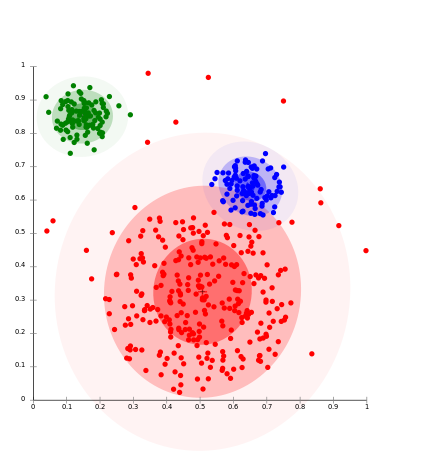
\includegraphics[width=5cm]{clustering.png}
    %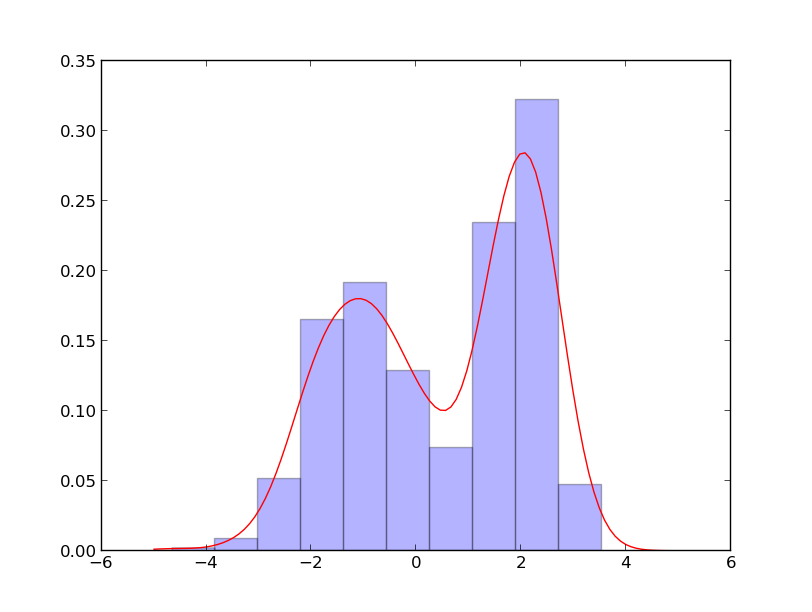
\includegraphics[width=6cm]{kerneldist.png}
    %\end{figure}
    %}

\begin{frame} {Which Face Is fake?}

    \begin{figure}
    \centering
    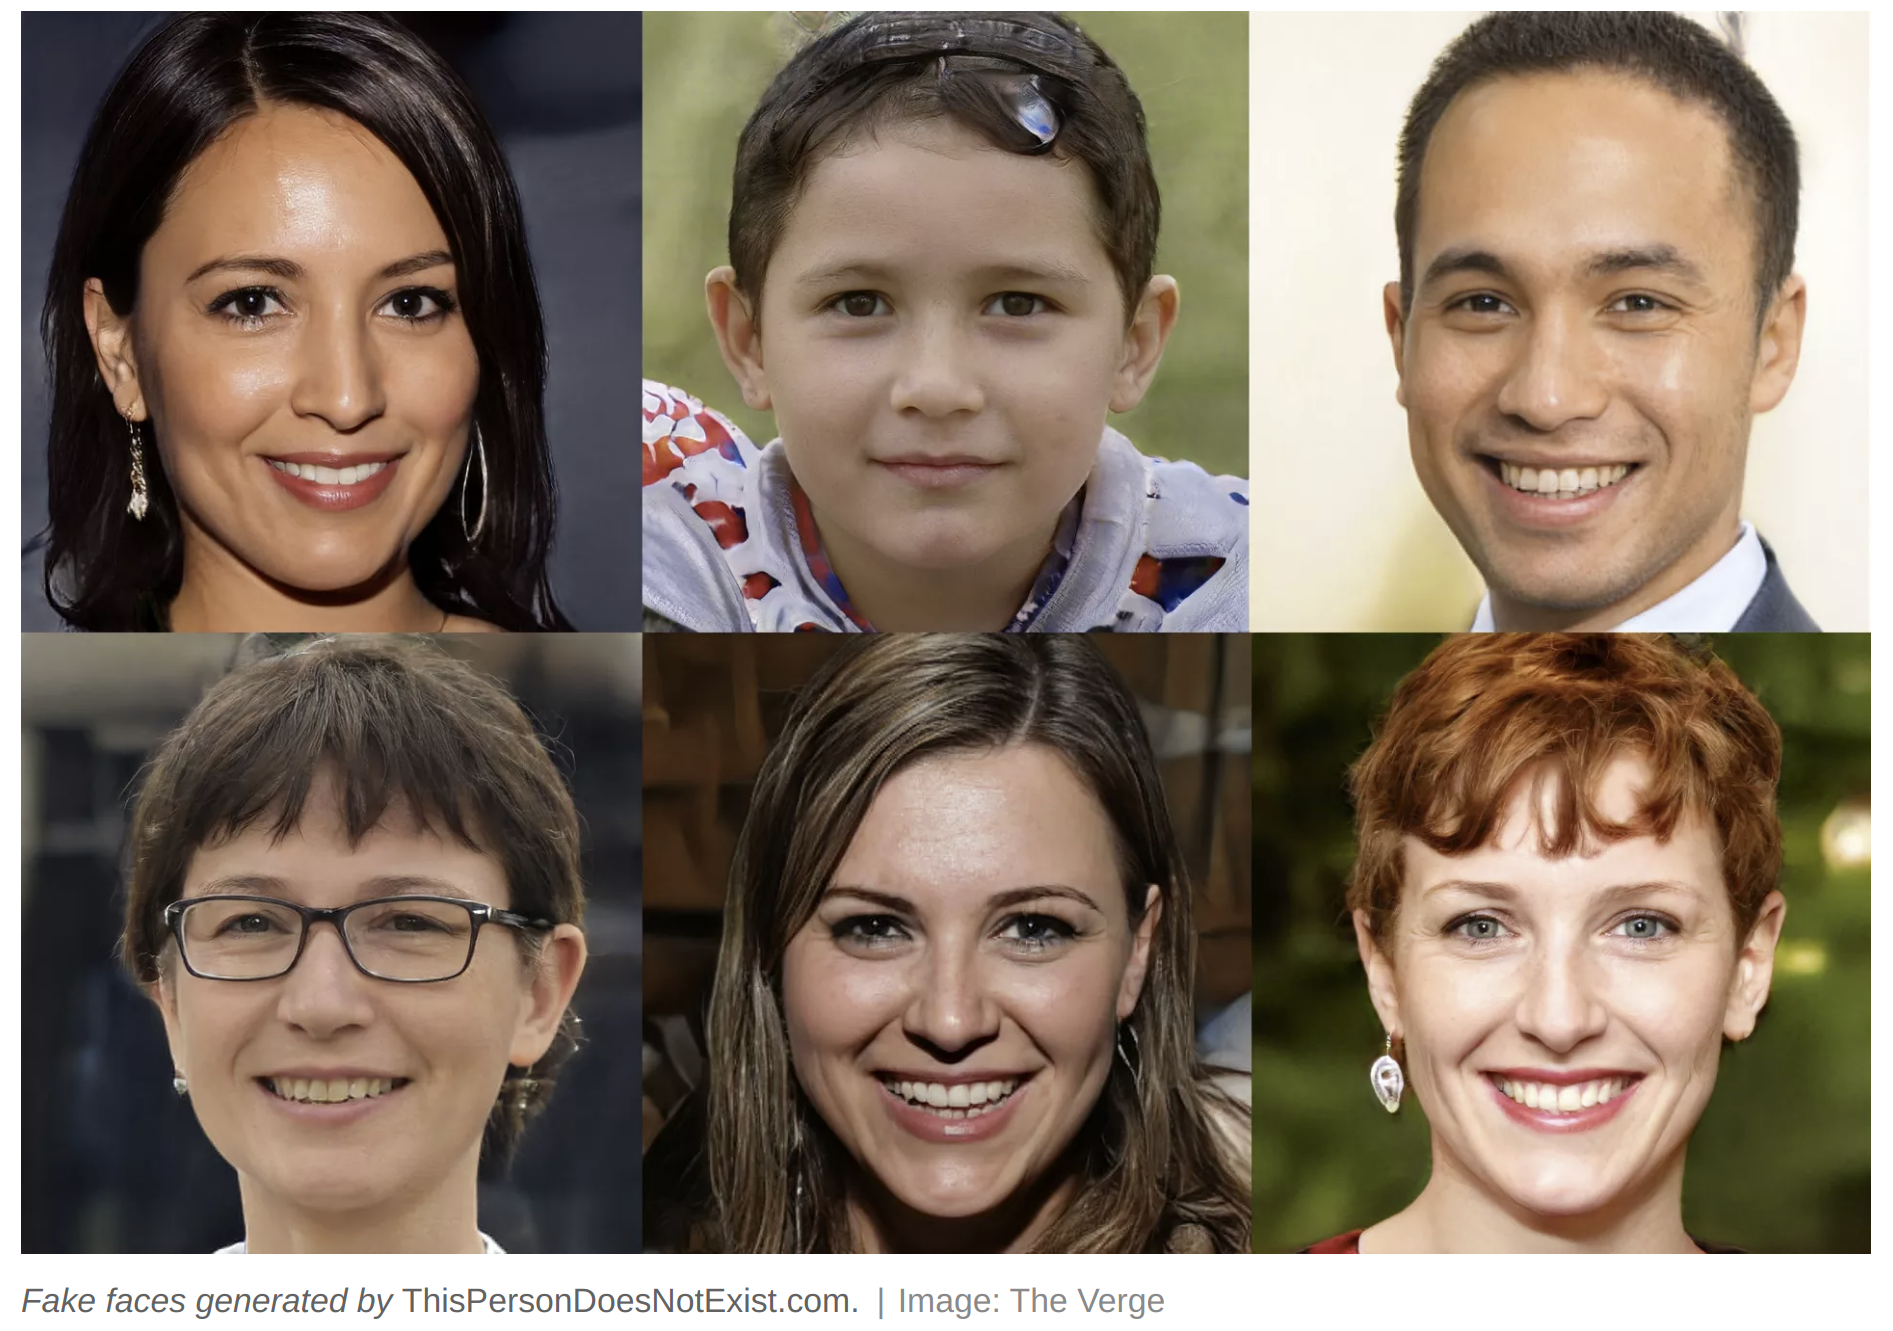
\includegraphics[width=10cm]{plots/exampleGAN.png}
    \end{figure}

\end{frame}

%\section{Supervised Learning vs Unsupervised Learning}


%\begin{frame} {Supervised Learning vs Unsupervised Learning }
%    \begin{itemize}
%    \item \textbf{Supervised Learning}
%    \item [$ $] \textbf{Data:} ($x , y$)
%    \item [$ $] $x$ is Data and $y$ is corresponding label
%    \item [$ $] \textbf{Goal:} learn function to map $x \rightarrow y$
%    \item [$ $] \textbf{Examples:} Classification, Regression, Object Detection, Image Segmentation, etc.
%    \end{itemize}
%    
%     \begin{itemize}
%    \item \textbf{Unsupervised Learning}
%    \item [$ $] \textbf{Data:} $x$
%    \item [$ $] $x$ is Data and no labels!
%    \item [$ $] \textbf{Goal:} learn hidden structure of data
%    \item [$ $] \textbf{Examples:} Clustering, Dimentionality Reduction, etc.
%    \end{itemize}
%
%\end{frame}



\begin{frame} {Deep Unsupervised Learning}
There are two main goals of \textbf{deep unsupervised learning}:
    \begin{itemize}
%\vspace{4mm}
\item \textbf{Representation Learning}
\begin{itemize}
\item Examples are: manifold learning, feature learning, etc.
\item Can be done by an autoencoder
\item Examples of applications:
    \begin{itemize}
\item dimensionality reduction / data compression
\item transfer learning / semi-supervised learning
\end{itemize}
\end{itemize}
%\vspace{2mm}
\item \textbf{Generative Models }
\begin{itemize}
\item Given a training set $\D = (\xi[1], \ldots, \xi[n])$ where each $\xi \sim \P_x$, the goal is to estimate $\P_x$.
\item \textbf{Goal:} Take as input training samples from some distribution and learn a model that represents that distribution!
\item Examples of applications:
    \begin{itemize}
\item generating music, videos, volumetric models for 3D printing, synthetic data for learning algorithms, outlier identification, images denoising, inpainting, etc.
\end{itemize}
\end{itemize}
\end{itemize}
\end{frame}

%\section{Generative Model}

\begin{frame}{Density Fitting / Learning a Generative Model}


Given  $\D = \left(\xi[1], \xi[2],\dots, \xi[n] \right) \sim \P_x$ learn a model of $\P_x$ (for example, fitting a Gaussian distribution via Maximum Likelihood Estimation). 

\only<1>{
    \begin{figure}
    \hspace{-5cm}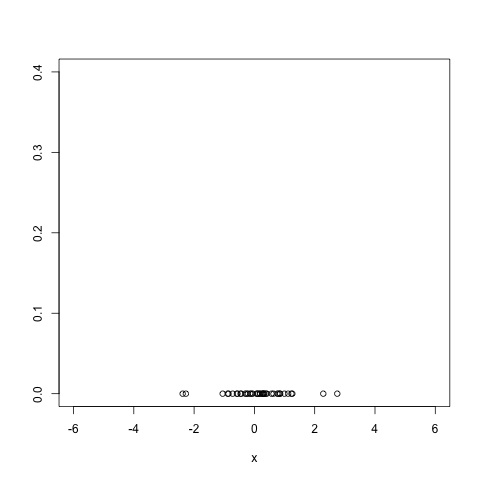
\includegraphics[width=5cm]{plots/sample.png}
    %\includegraphics[width=6cm]{sample-withGaussian.png}
    \end{figure}
}
\pause
\only<2>{
    \begin{figure}
    \centering
    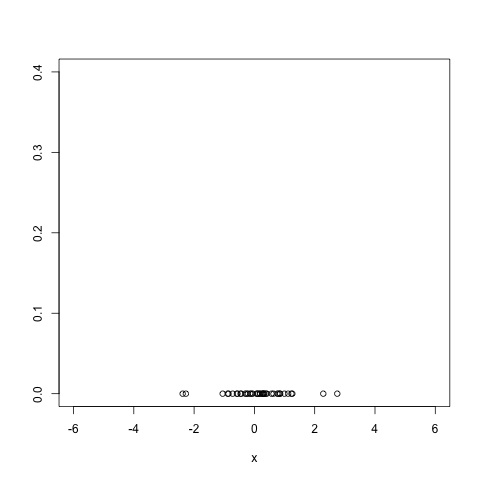
\includegraphics[width=5cm]{plots/sample.png}
    \includegraphics[width=5cm]{plots/sample-withGaussian.png}
    \end{figure}
}

\end{frame}

%\section{Application of Generative Model}

\begin{frame}{Why generative models?}
    
    Generative model are capable of uncovering underlying latent variables in a dataset and
        %is a probabilistic model  of the data generating distribution $p_{data}$.
    %It
    can be used for
    
    \begin{itemize}
    \item sampling / data generation
    \item outlier detection
    \item missing feature extraction
    \item image denoising / reconstruction
    \item representation learning
    \item planning in reinforcement learning
    \item ...
    \end{itemize}
    
\end{frame}


\begin{frame} {Application Example: Image generation}
    
        \vspace{8mm}
    \begin{figure}
    \centering
    \scalebox{1}{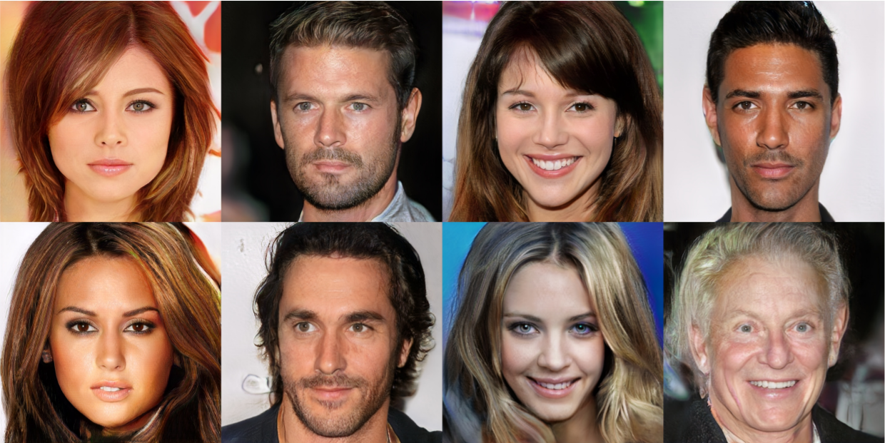
\includegraphics{plots/fake_celeb.png}}
    \tiny{\\Source: Karras et al. (2018)}
    \caption{Synthetic faces generated by a Generative Adversarial Network (more on this later).}
    \end{figure}

\end{frame}

\begin{frame} {Application Example: Neural Style Transfer}
    
    A photograph is \enquote{redrawn} in the style of another image! (Gatys et al., 2015) 
        \vspace{8mm}
    \begin{figure}
    \centering
    \only<1>{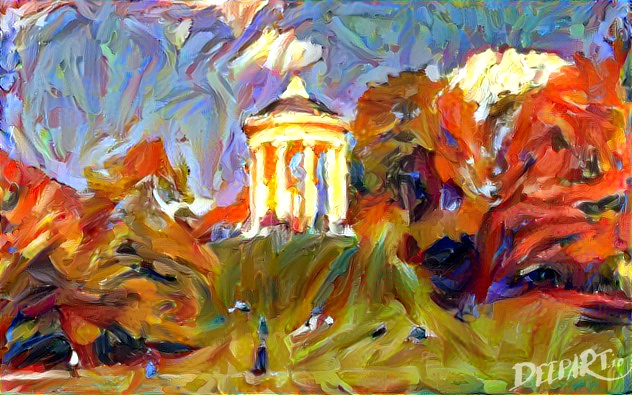
\includegraphics[width=0.33\textwidth]{plots/styletransfer_monopteros1.jpg} ~~ 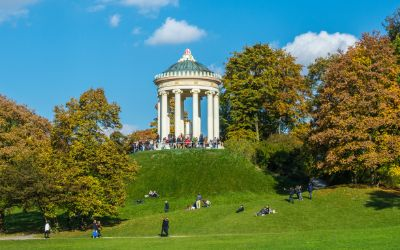
\includegraphics[width=0.33\textwidth]{plots/styletransfer_monopteros.jpg}~~\includegraphics[width=0.2\textwidth]{plots/styletransfer1.jpg}}
    \only<2>{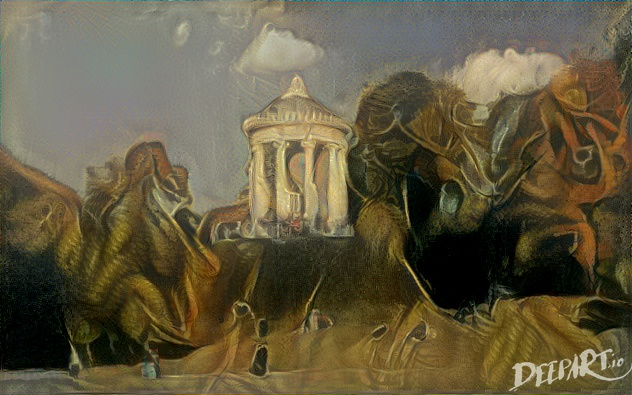
\includegraphics[width=0.33\textwidth]{plots/styletransfer_monopteros2.jpg} ~~ 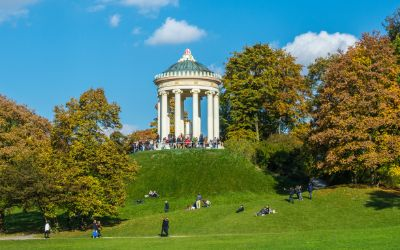
\includegraphics[width=0.33\textwidth]{plots/styletransfer_monopteros.jpg}~~\includegraphics[width=0.2\textwidth]{plots/styletransfer2.jpeg}}
    \only<3>{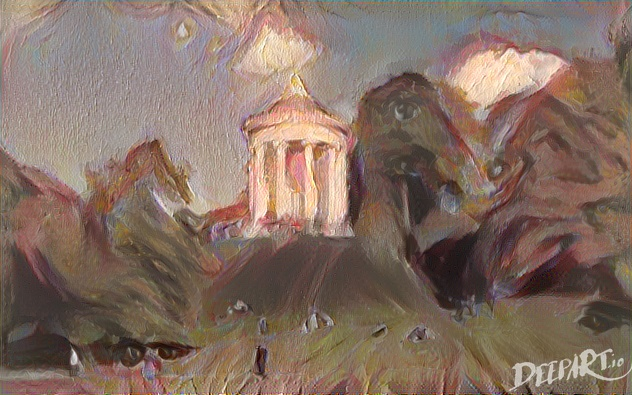
\includegraphics[width=0.33\textwidth]{plots/styletransfer_monopteros3.jpg} ~~ 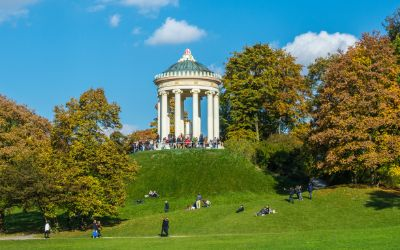
\includegraphics[width=0.33\textwidth]{plots/styletransfer_monopteros.jpg}~~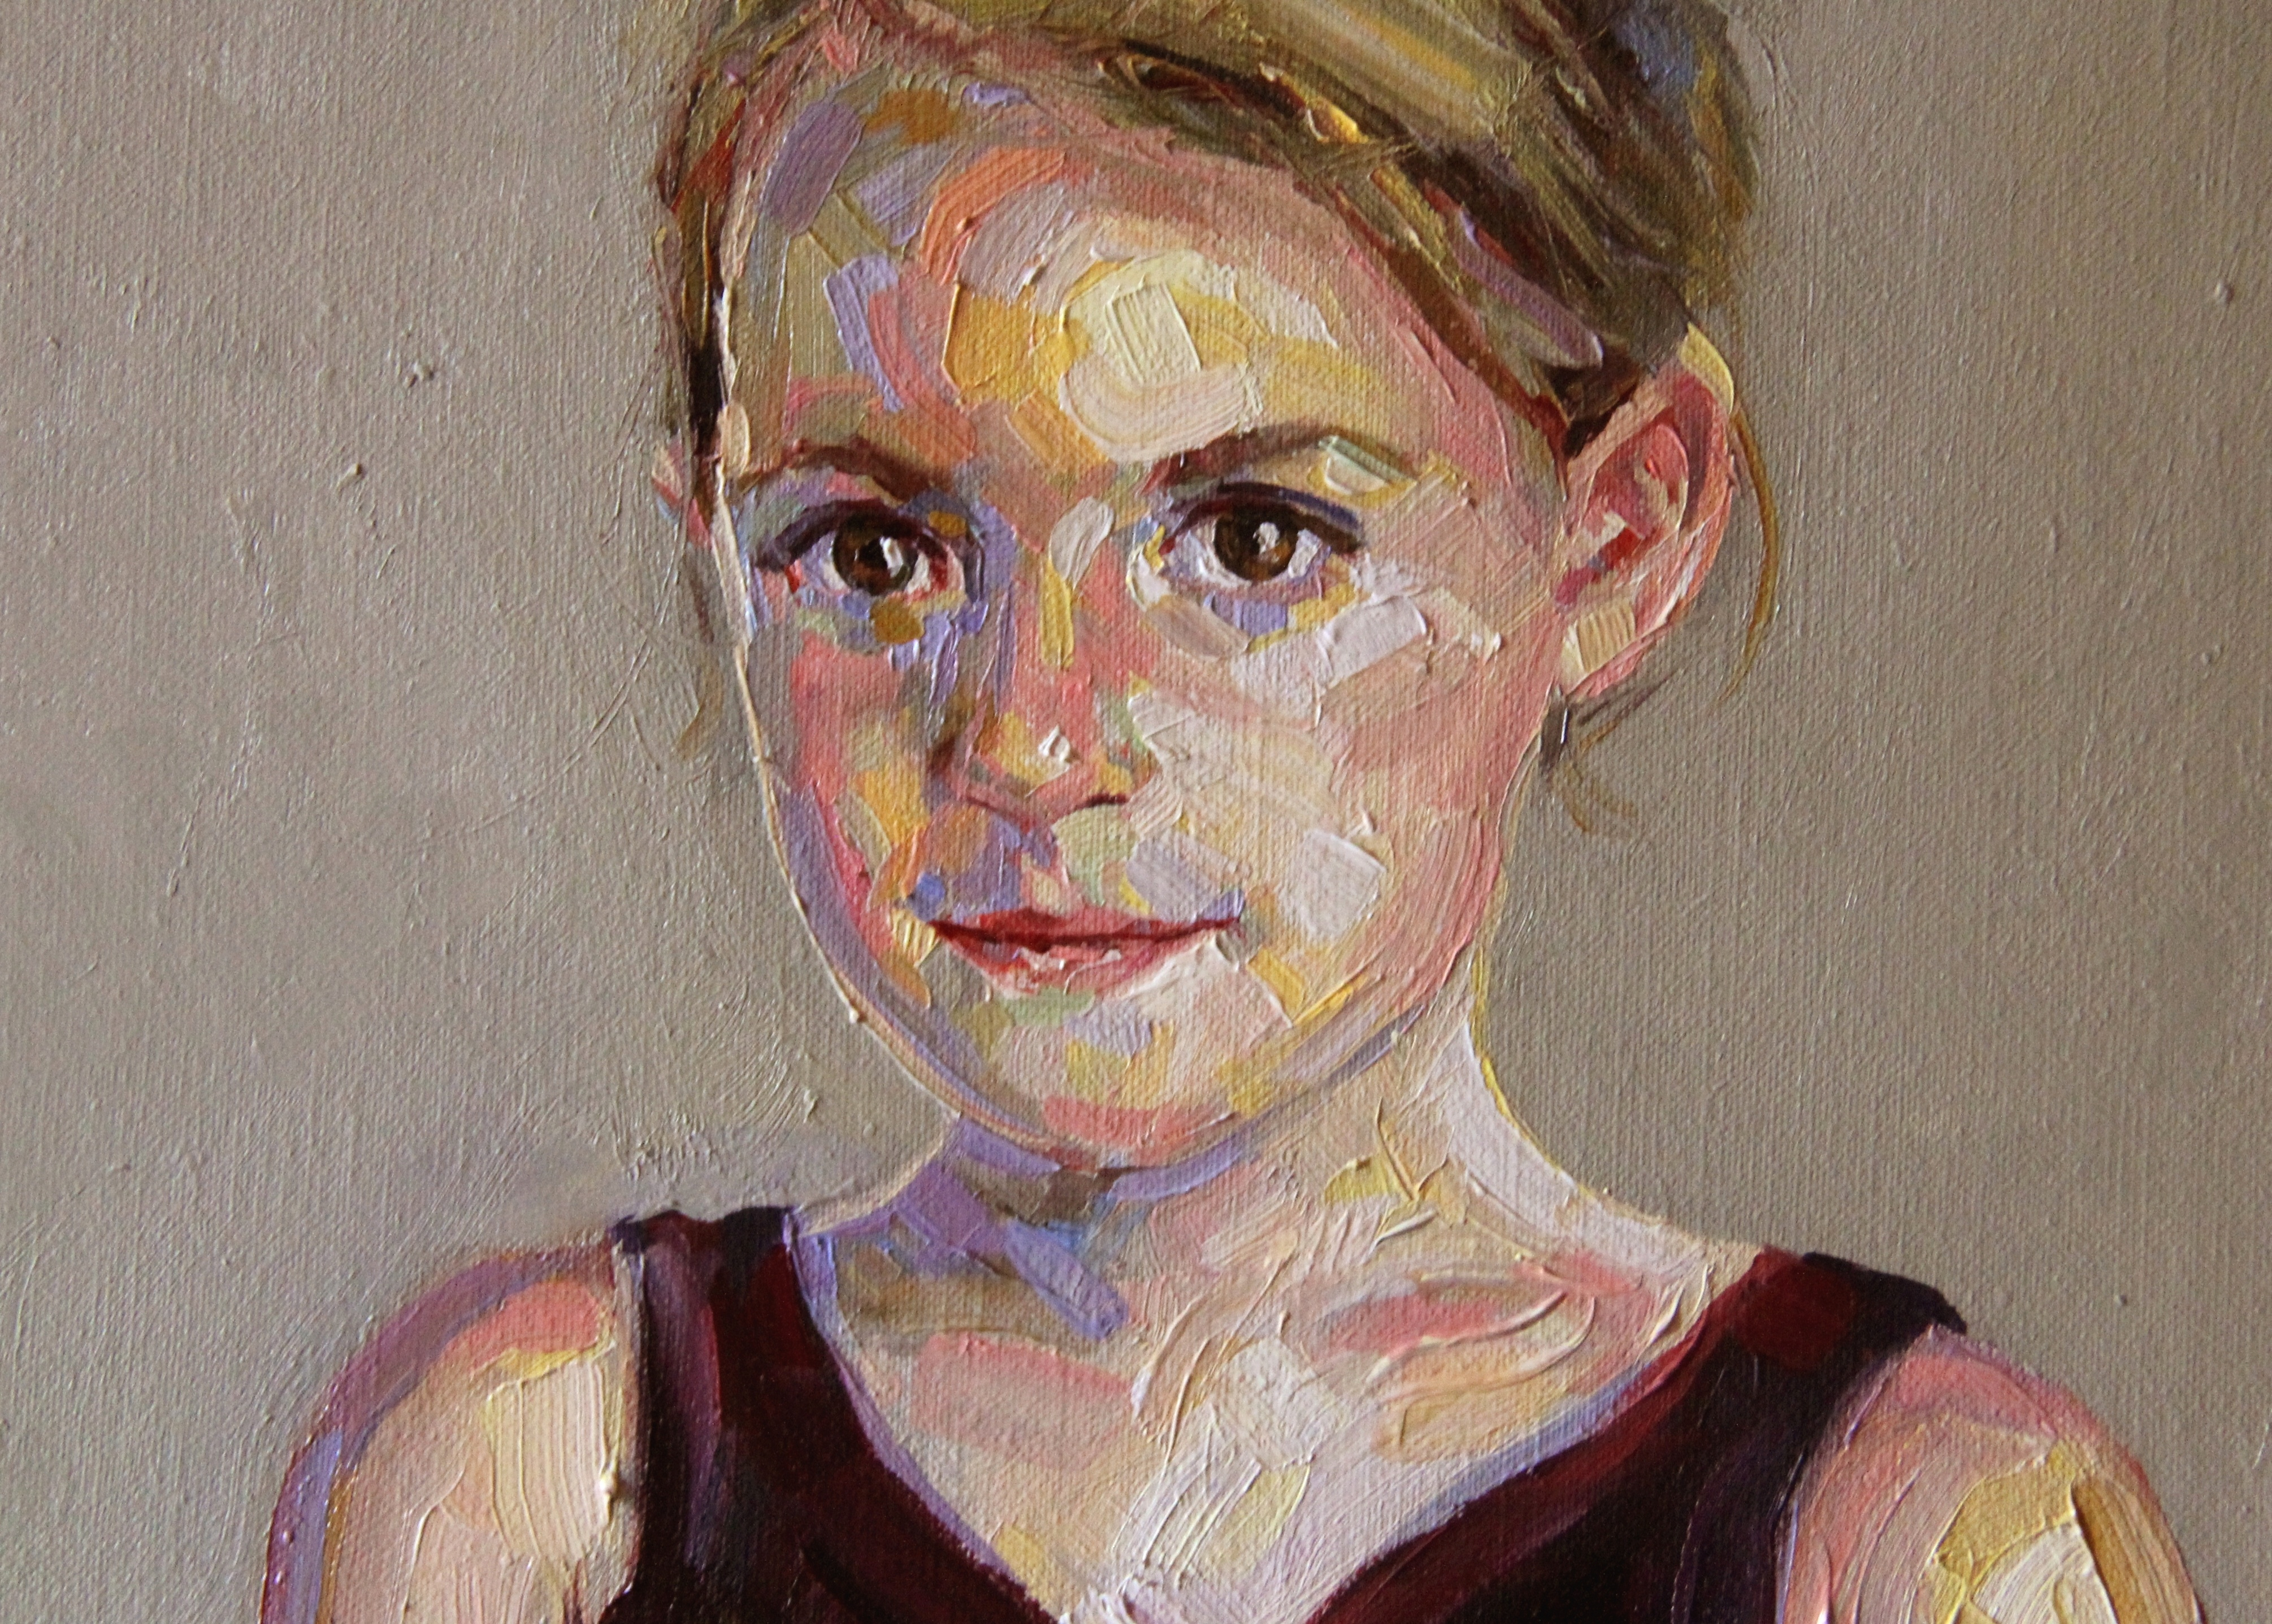
\includegraphics[width=0.25\textwidth]{plots/styletransfer3.jpg}}
    \caption{Examples generated on \url{https://deepart.io/}. The image on the left has been generated by translating the original image (middle) to the style of the image on the right. }
    \end{figure}

\end{frame}


\begin{frame} {Application Example: Image Inpainting}

    \vspace{8mm}
    \begin{figure}
    \centering
    \scalebox{1}{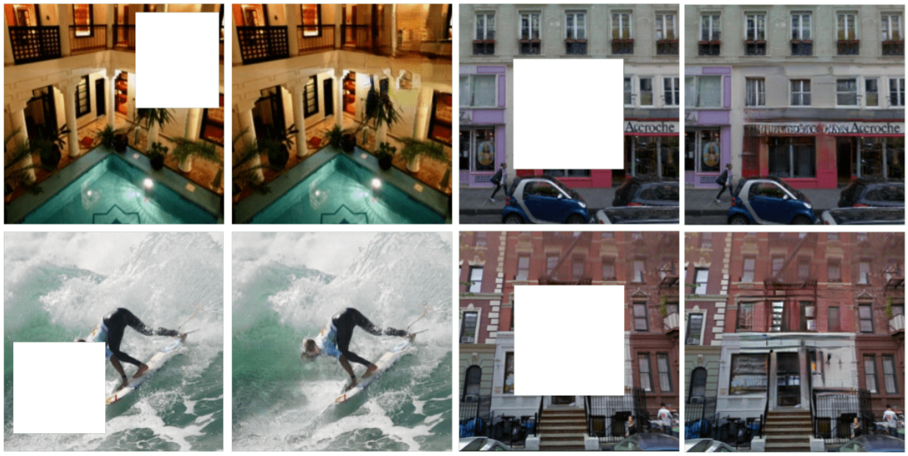
\includegraphics{plots/inpainting.png}}
    \tiny{\\Source: Demir et al (2018)}
    \caption{A generative model fills in the missing portion of the image based on the surrounding context.}
    \end{figure}

\end{frame}





 \begin{frame} {Application Example: Semantic Labels --> Images}

     \begin{figure}
     \centering
     \scalebox{1}{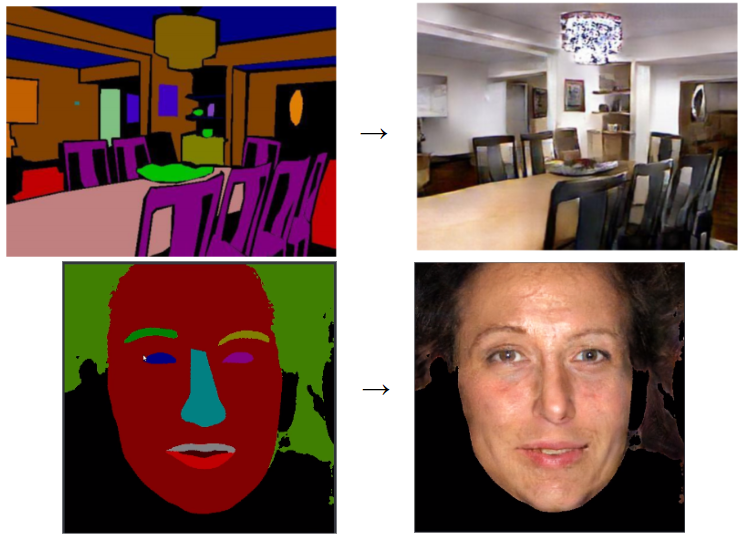
\includegraphics{plots/sem_to_img.png}}
     \tiny{\\Source: Wang et al (2017)}
     \end{figure}

 \end{frame}


 \begin{frame} {Application Example: Generating Images from Text}
   
     \begin{figure}
     \centering
     \scalebox{1}{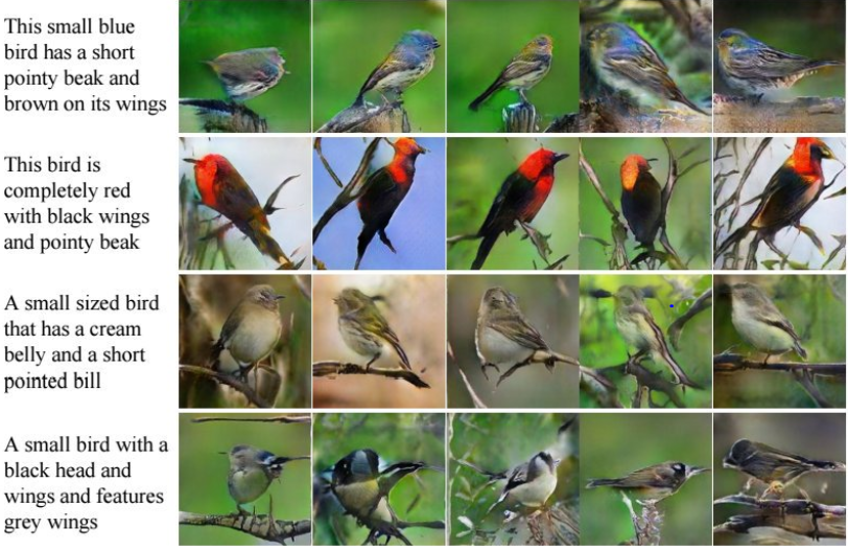
\includegraphics{plots/text_to_img.png}}
     \tiny{\\Source: Zhang et al (2017)}
     \end{figure}

 \end{frame}



%\frame{\frametitle{Outline}\tableofcontents}
% \AtBeginSubsection[]
% {
    %   \begin{frame}
    %       \frametitle{Outline}
    %       %\tableofcontents[currentsection,currentsubsection]
    %       \tableofcontents[currentsection]
    %   \end{frame}
    %}

%%%%%%%%%%%%%%%%%%%%%%%%%%%%%%%%%%%%%%%%%%%%%%%%%%%%%%%%%%%%%%%%%%
%%%%%%%%%%%%%%%%%%          REFERENCES          %%%%%%%%%%%%%%%%%%
%%%%%%%%%%%%%%%%%%%%%%%%%%%%%%%%%%%%%%%%%%%%%%%%%%%%%%%%%%%%%%%%%%
\begin{vbframe}
\frametitle{References}
\footnotesize{
\begin{thebibliography}{99}
%%%%%%%%%%%%%%%%%%%%%%%%%%%%%%%%%%
\bibitem[Demir et al., 2018]{3} Ugur Demir, Gozde Unal (2018)
\newblock Patch-Based Image Inpainting with Generative Adversarial Networks
\newblock \emph{\url{https://arxiv.org/abs/1803.07422}}
%%%%%%%%%%%%%%%%%%%%%%%%%%%%%%%%%%
%%%%%%%%%%%%%%%%%%%%%%%%%%%%%%%%%
\bibitem[Karras et al., 2018]{4} Tero Karras, Timo Aila, Samuli Laine, Jaakko Lehtinen (2018)
\newblock Progressive Growing of GANs for Improved Quality, Stability, and Variation
\newblock \emph{\url{https://arxiv.org/abs/1710.10196}}
%%%%%%%%%%%%%%%%%%%%%%%%%%%%%%%%%%
%%%%%%%%%%%%%%%%%%%%%%%%%%%%%%%%%
\bibitem[Gatys, 2015]{14} Leon A. Gatys et al. (2015)
\newblock Neural Algorithm of Artistic Style
\newblock \emph{\url{https://arxiv.org/abs/1508.06576}}



\end{thebibliography}
}
\end{vbframe}
%%%%%%%%%%%%%%%%%%%%%%%%%%%%%%%%%%%%%%%%%%%%%%%%%%%%%%%%%%%%%%%%%%
%%%%%%%%%%%%%%%%%%%%%%%%%%%%%%%%%%%%%%%%%%%%%%%%%%%%%%%%%%%%%%%%%%

\endlecture
\end{document}
